\documentclass[a4paper,german,12pt,smallheadings]{scrartcl}
\usepackage[T1]{fontenc}
\usepackage[utf8]{inputenc}
\usepackage{babel}
\usepackage{geometry}
\usepackage[fleqn]{amsmath}
\usepackage{amssymb}
\usepackage{float}
\usepackage{enumerate}
\usepackage{commath} % http://tex.stackexchange.com/questions/14821/whats-the-proper-way-to-typeset-a-differential-operator
\usepackage{cancel}
\usepackage{pdfpages}

\usepackage[fleqn]{mathtools}
% Number only referenced equations
%\mathtoolsset{showonlyrefs}

%\usepackage{wrapfig}
\usepackage[thinspace,thinqspace,squaren,textstyle]{SIunits}
\usepackage{tikz}
\usepackage[europeanresistors]{circuitikz}

% New command for color underlining
\usepackage{xcolor}

\newsavebox\MBox
\newcommand\colul[2][red]{{\sbox\MBox{$#2$}%
  \rlap{\usebox\MBox}\color{#1}\rule[-1.2\dp\MBox]{\wd\MBox}{0.5pt}}}

\restylefloat{table}
\geometry{a4paper, top=15mm, left=20mm, right=10mm, bottom=20mm, headsep=10mm, footskip=12mm}
\linespread{1.5}
\setlength\parindent{0pt}
\DeclareMathOperator{\Tr}{Tr}
\DeclareMathOperator{\Var}{Var}
\begin{document}
\allowdisplaybreaks % Seitenumbrüche in Formeln erlauben
\begin{center}
\bfseries % Fettdruck einschalten
\sffamily % Serifenlose Schrift
\vspace{-40pt}
Physikalisches Grundpraktikum 2, Wintersemester 2014/2015

Markus Fenske \texttt{<iblue@zedat.fu-berlin.de>}

Transistor, Tutor: Andreas Maier
\vspace{-10pt}
\end{center}
\section{Einführung}
Ziel des Versuches ist die Aufnahme des Kennlinienfeldes eines
npn-Bipolartransistors  Außerdem soll eine Verstärkerstufe mit
Parallel-Gegenkopplung aufgebaut und die Verstärkung mit den theoretischen
Erwartungen verglichen werden.

\section{Theoretische Grundlagen}

\subsection{Transistor}

Der Transistor ist ein elektronisches Bauelement bei dem der Stromfluss auf
einer Strecke (Kollektor-Emitter) durch den Stromfluss auf der anderen Strecke
(Basis-Emmitter) gesteuert werden kann. Der Name leitet sich von
\textit{tran}sfer re\textit{sistor} ab, also einem steuerbaren Widerstand.

\subsubsection{Aufbau}

Anlog zur Diode handelt es sich um einen Aufbau aus dotierten Halbleitern
(Erklärung siehe dort). Im Unterschied zur Diode werden beim hier verwendeten
Transistor eine n-dotierte Schicht an eine p-dotierte Schicht und dann wieder
an eine n-dotierte Schicht gebracht. Es entstehen also zwei
Rekombinationszonen. Die n-dotierten Seiten heißen Kollektor und Emitter, die
p-Schicht in der Mitte Basis.

% FIXME: Grafik!
Wird der Transistor nun mit Kollektor und Emitter angeschlossen, leitet er in
keine Richtung, denn die Schaltung entspricht prinzipiell zwei gegeneinander
verschalteten Dioden. Die eine Sperrschicht wird zwar (bei genügend großer
Spannung) abgebaut, die andere jedoch vergrößert.

Betrachtet man den Betrieb in vorgesehener Richtung (Pluspol am Kollektor,
Minuspol am Emitter) ist nun also die Sperrschicht zwischen Basis und Emitter
abgebaut, die Sperrschicht zwischen Kollektor und Basis allerdings vergrößert.

Wir nun jedoch eine geringe Spannung zwischen Basis und Emitter angelegt,
beginnen Elektronen vom Emitter zur Basis zu fließen. Da die Sperrschicht
zwischen Basis und Kollektor jedoch klein ist und das Potential zwischen Basis
und Kollektor wesentlich größer ist, driften die meisten Elektronen direkt zum
Kollektor. Es fließt nun also ein Strom zwischen Kollektor und Emitter, der
Transistor leitet.

\subsubsection{Kennlinienfeld}

Die grundlegenden quantitativen Eigenschaften eines Transistors lassen sich im
Kennlinienfeld zusammenfassen. Es setzt die Ströme und Spannungen am Transistor
in Relation. Am Transistor lassen sich drei Spannungen messen. Die Spannung
zwischen Kollektor und Emitter ($U_{CE}$), die Spannung zwischen Basis und
Emitter ($U_{BE}$) und die Spannung zwischen Kollektor und Basis ($U_{CB}$). Da
das elektrische Feld konservativ ist, gilt

\begin{equation}
  U_{CE} = U_{CB} + U_{BE}
\end{equation}

Außerdem lassen sich die Ströme an Basis, Emitter und Kollektor messen.
Aufgrund der Ladungserhaltung gilt dann

\begin{equation}
  I_C + I_B + I_E = 0
\end{equation}

Somit bleiben vier freie Parameter, die durch das Kennlinienfeld jeweils in
Relation gesetzt werden, um das Verhalten des Transistors zu beschreiben.

\begin{figure}[H]
  \centering
  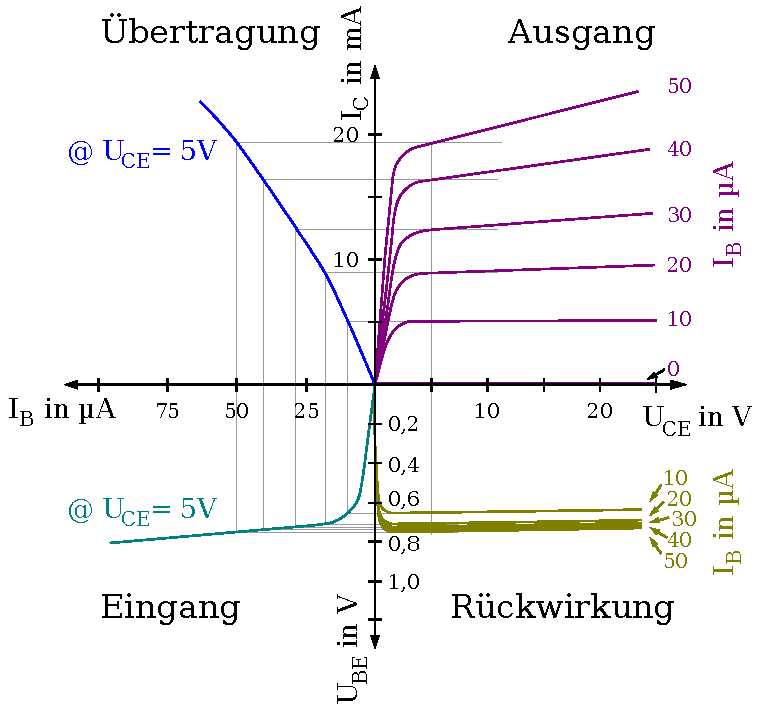
\includegraphics[width=.6\textwidth]{kennlinienfeld.pdf}
  \label{img:kennlinie}
  \caption{Kennlinienfeld eines Transistors}
\end{figure}

Im ersten Quadranten lässt sich der \textit{Ausgangswiderstand} ablesen. Er
gibt das Verhältnis Emitter-Kollektor-Spannung $U_{CE}$ und dem Kollektorstrom
$I_C$ an.

Im zweiten Quadranten wird das Stromsteuer-, Übertragungs- oder auch
Stromverstärkungskennlinienfeld dargestellt. Es setzt Basis- und Kollektorstrom
in Relation und bestimmt damit den Verstärkungsfaktor.

Im dritten Quadranten lässt sich der Eingangswiderstand ablesen. Er gibt das
Verhältnis zwischen Basis-Emitter-Spannung $U_{BE}$ und Basisstrom $I_B$ an.

Im vierten Quadranten ist die Spannungsrückwirkung aufgetragen, sie gibt das
Verhältnis der beiden obigen Spannungen an.

Oft wird ins Kennlinienfeld auch die \textit{Leistungshyperbel} aufgetragen.
Der Ausgangswiderstand des Transistors führt nämlich zu einer Verlustleistung
und damit zur Erwärmung des Transistors. Um eine Überhitzung zu vermeiden, darf
die Leistung eine Grenze $P = UI$ nicht überschreiten. Trägt man $I$ in
Abhängigkeit von $U$ bei konstanten $P$ auf, ergibt sich somit eine Hyperbel.

\begin{equation}
  U(I) = \frac{P}{I}
\end{equation}

Der Aufbau zur Aufnahme des Kennlinienfeldes ist in der folgenden Abbildung
dargestellt. Es kann der Basisstrom und die Emitter-Kollektor-Spannung variiert
werden, um die jeweiligen Parameter aufzunehmen.

\begin{figure}[H]
  \begin{center}
    \begin{circuitikz}
      \draw (0,0)
      to[battery1=$1{,}5V$] (0,2)
      to[ammeter,l=$I_B$] (2,2)
      to[R=$2{,}2\;\text{k}\Omega$] (4,2)
      to[vR=$22\;\text{k}\Omega\;\text{(log)}$] (6,2)
      to[voltmeter,l=$U_{EB}$] (6,0)
      to[short] (0,0);
      \draw (8,2) node[npn] (npn) {}
      (npn.base) node[anchor=south] {B}
      (npn.collector) node[anchor=west] {C}
      (npn.emitter) node[anchor=west] {E};
      \draw (6,2) |- (npn.base);
      \draw (6,0) -| (npn.emitter);
      \draw (6,0)
      to[short] (12,0)
      to[V,v=$U_0$] (12,6)
      to[short] (10,6)
      to[ammeter,l=$I_C$] (10,3.5)
      -| (npn.collector);
      \draw (10,4)
      to[voltmeter,l=$U_{EC}$] (10,0);
    \end{circuitikz}
    \caption{Aufbau zur Messung des Kennlinienfeldes}
  \end{center}
\end{figure}

\subsubsection{Verstärkerschaltung}

Möchte man eine Wechselspannung verstärken, müssen einige Maßnahmen zur
Signalanpassung getroffen werden. Da der Transistor nur positive
Basis-Emitter-Ströme verstärkt, muss das Potential des Signals angehoben
werden. Wird der erreichte Punkt im Kennlinienfeld dargestellt, spricht man von
Arbeitspunkt.

Um nur Wechselspannungen zu verstärken, wird das Signal jeweils durch
einen Koppelkondensator an Ein- und Ausgang gefiltert.

Da Halbleiter stark temperaturabhängig sind, möchte man den Arbeitspunkt
stabilisieren um ein gleichmäßiges Verhalten bei unterschiedlichen Temperaturen
zu erreichen. Dazu nutzt man die \textit{Gegenkopplung}. Dabei wird ein Teil
des Ausgangsstroms über einen Widerstand zurückgeführt um den Arbeitspunkt
entsprechend zu verschieben. Ist der Emitterstrom bei höherer Temperatur
größer, senkt dies den Arbeitspunkt auf einen geringeren Wert (siehe Schaltung).

\begin{figure}[H]
  \begin{center}
    \begin{circuitikz}
      \draw (4,2) node[npn] (npn) {}
      (npn.base) node[anchor=south] {B}
      (npn.collector) node[anchor=west] {C}
      (npn.emitter) node[anchor=west] {E};
      \draw (0,2)
      to[C=$C_k$] (1.5,2) % Bisschen Platz machen, sonst label kaputt.
      to[short]   (2,2)
      to[short] (npn.base);
      \draw (0,0) -| (npn.emitter) |- (6,0);
      \draw (2,2)
      to[R=$R_V$] (2,4)
      to[short] (4,4) |- (npn.collector);
      \draw (4,4)
      to[C=$C_k$] (6,4);
      \draw (4,4)
      to[R=$R_A$] (4,6)
      to[short] (6,6);
      \draw (6,6) node[anchor=west] {12V};
      \draw (6,4) node[anchor=west] {Aus};
      \draw (6,0) node[anchor=west] {0V};
      \draw (0,2) node[anchor=east] {Ein};
      \draw (0,0) node[anchor=east] {0V};
    \end{circuitikz}
    \caption{Verstärkerschaltung mit Gegenkopplung}
  \end{center}
\end{figure}

\section{Aufgaben}
\begin{enumerate}
  \item Aufnahme und Konstruktion des statischen Kennlinienfeldes eines
    npn-Transistors bei einer Versorgungsspannung von 12V. Bestimmung der
    Stromverstärkung für den statischen Fall.
  \item Aufbau einer Verstärkerschaltung mit Parallelgegenkopplung und
    Verstärkung einer Eingangswechselspannung.
\end{enumerate}


\end{document}
